%!Tex Program = pdflatex
\documentclass[12pt,a4paper]{report}

\usepackage{preamble}

\begin{document}

\input{titlepage}

\input{certificate}

\newpage
\noborders
\pagestyle{myfooters}
\pagenumbering{roman}
\phantomsection
\begin{center}
	\Large{\textbf{Abstract}}
\end{center}
\addcontentsline{toc}{chapter}{Abstract}
\par This paper presents the development and implementation of an innovative attendance monitoring system leveraging facial recognition technology. The conventional methods of attendance tracking often suffer from inaccuracies, inefficiencies, and susceptibility to fraudulent practices. To address these challenges, we propose a robust solution that harnesses the power of facial recognition to accurately identify individuals and record their attendance seamlessly. The system architecture consists of three main components: face detection, face recognition, and attendance management. The face detection module employs advanced computer vision techniques to locate and extract facial features from input images. Subsequently, the face recognition module utilizes machine learning algorithms, to match detected faces against a database of known individuals, thereby ensuring accurate identification. Furthermore, the attendance management component facilitates the storage and organization of attendance records in a centralized database, enabling administrators to monitor and analyze attendance data efficiently. Additionally, the system offers real-time monitoring capabilities, allowing administrators to track attendance remotely and receive instant notifications for any irregularities or unauthorized access attempts. The proposed attendance monitoring system offers numerous advantages, including improved accuracy, enhanced security, and streamlined administrative processes. By leveraging facial recognition technology, organizations can mitigate the shortcomings associated with traditional attendance tracking methods, thereby optimizing operational efficiency and fostering a more secure and transparent environment.

\newpage
\noborders
\phantomsection
\begin{center}
	\Large{\textbf{Acknowledgement}}
\end{center}
\addcontentsline{toc}{chapter}{Acknowledgement}
%ACKNOWLEDGEMENT
\begin{flushright}
	\textbf{NAME\\}
\end{flushright}

\newpage
\noborders
\tableofcontents
\addcontentsline{toc}{chapter}{Table of Contents}

\newpage
\noborders
\listoffigures

\newpage
\noborders
\pagestyle{plain}
\pagenumbering{arabic}

\chapter{Introduction}
\section{Introduction}
\par The project leverages facial recognition technology to automate attendance management. Using a combination of a Raspberry Pi Pico WH microcontroller and a Python-based GUI, the system allows for seamless student registration, attendance marking, and database management. This report outlines the project's components, setup, and usage instructions.\\
\par The Attendance Monitoring System Using Facial Recognition is an innovative solution designed to enhance the accuracy, efficiency, and security of attendance management processes. This system leverages advanced biometric technology to identify and verify individuals based on their unique facial features. By employing high-resolution cameras and sophisticated facial recognition algorithms, the system captures real-time images of individuals and matches them against a pre-enrolled database to record their attendance automatically.\\
\par The primary components of the system include facial recognition software, a secure database for storing facial data and attendance records, and a user-friendly interface for administrators and users. The system operates by enrolling individuals through an initial capture of their facial images, which are then stored in the database. Upon subsequent encounters, the system performs real-time facial recognition to identify the individuals and log their attendance accurately.\\
\par Key benefits of this system include the elimination of manual errors, enhanced security by preventing unauthorized access, and significant time savings compared to traditional methods. The system's applications span across educational institutions, workplaces, and events, where it streamlines the process of attendance tracking and provides comprehensive reports and analytics.\\
\par OpenCV (Open Source Computer Vision Library) is an open-source computer vision and machine learning software library. It contains more than 2500 optimized algorithms for various tasks like image processing, computer vision, and machine learning. Some of the key features are, image processing where functions for filtering, edge detection, and image transformations, video analysis with tools for object detection and tracking. Face recognition is a technology capable of identifying or verifying a person from a digital image or a video frame. OpenCV, along with other libraries like dlib, is commonly used for face recognition tasks.\\
\par The Raspberry Pi Pico WH is a microcontroller board based on the RP2040 microcontroller chip. It's designed for physical computing projects and is popular in the maker community. It's key features involves having a RP2040 microcontroller with Dual-core ARM Cortex-M0+ processor, connectivity of 2.4 GHz wireless connectivity (WiFi), GPIO with 26 multifunction pins, programmed using MicroPython, C/C++, and CircuitPython.\\
\par Overall, the Attendance Monitoring System Using Facial Recognition represents a significant advancement in attendance management, offering a reliable, secure, and efficient alternative to conventional methods. This technology not only simplifies administrative tasks but also ensures precise and tamper-proof attendance records.

\section{Background Information}
\par An attendance monitoring system using facial recognition and IoT integrates cutting-edge technologies to automate and improve attendance recording in settings like schools, workplaces, and events. This system employs facial recognition to accurately identify individuals and IoT devices to facilitate the seamless capture, processing, and transmission of data.\\
\par Imagine a school or workplace where taking attendance is quick, accurate, and effortless. That's the promise of using facial recognition technology combined with the Internet of Things (IoT) for attendance monitoring. This advanced system transforms the mundane task of roll call into a seamless, automated process.\\
\par At its core, the system uses high-resolution cameras to capture images of people as they walk into a room or building. Instead of manually checking names off a list, machine learning algorithms take over. These algorithms, similar to those used in your phone's face unlock feature, scan the captured images to recognize each person's face. They are smart enough to tell people apart, even in a crowd or under varying lighting conditions.\\
\par The role of IoT devices in this setup is vital. Think of these devices as the eyes and ears of the system. Cameras and sensors gather data continuously. This data is then processed locally by small, powerful edge computing devices, which act like mini-computers. These devices ensure that the system works swiftly without the delays that can come from sending all data to a remote server.\\
\par Once processed, the data is sent to cloud servers. The cloud is where the heavy lifting happens, storing all the images and attendance records securely. Cloud computing provides the necessary power and space to handle vast amounts of information. Additionally, secure databases keep this information safe and ensure it complies with privacy laws.\\
\par Finally, specialized software brings everything together. This software automates the attendance recording process, generating real-time reports and insights. Administrators can easily access this information, making the whole system efficient and user-friendly.\\
\par In short, combining facial recognition with IoT for attendance monitoring makes the process faster, more accurate, and far less manual. It's a step into the future, where technology takes care of the routine tasks, allowing people to focus on what truly matters.

\section{Research Gap}
\par Traditional attendance systems have faced a multitude of challenges, particularly in educational institutions and workplaces. These problems have prompted the need for more advanced solutions like facial recognition-based attendance systems. Some of the key issues are, viz.
\begin{enumerate}
	\item \textbf{Time-Consuming Processes} - Taking attendance manually is time-consuming, especially in larger areas. It disrupts the flow of activities and reduces productivity. Verifying and compiling attendance records can be slow.
	\item  \textbf{Lack of Real-Time Tracking} - Traditional systems do not provide real-time data, which can be critical for timely decision-making and monitoring. Due to lack of real-time updates leads to delays in identifying absentees and taking necessary actions.
	\item \textbf{Inefficiency in Large Scale Management} - As the number of attendees increases, managing and maintaining accurate records becomes increasingly difficult, and Requires significant resources for managing and maintaining attendance records, leading to higher operational costs.
	\item \textbf{Security} - Providing the security for the data which is monitored will be most challenging phase while monitoring the attendance.
\end{enumerate}

\section{Problem Statement}
\par Attendance Management System is software developed for daily student attendance in schools, colleges and institutes. It facilitates to access the attendance information of a particular student in a particular class. This system will also help in evaluating attendance eligibility criteria of a student. By just a click on the mouse, the system will be able to produce the students' attendance report thus reducing the need of time consumption.\\
\par This application is built for automating the processing of attendance. It also enhances the speed and enhances the accuracy.\\
\par In educational institutions, workplaces, and events, the traditional methods of tracking attendance are fraught with inefficiencies and inaccuracies. Manual systems, which involve manually checking off names on a list or using sign-in sheets, are labor-intensive and prone to human error. Administrators spend significant amounts of time on these tasks, which could be better spent on more productive activities. Furthermore, these methods are vulnerable to fraudulent practices, such as proxy attendance, where one person signs in for another.\\
\par RFID and card-based systems were introduced as a solution to some of these problems. However, they come with their own set of challenges. Employees and students often forget or lose their cards, leading to delays and administrative headaches. These systems also do not completely eliminate the possibility of misuse, as cards can be shared among individuals. Additionally, they still require some degree of manual intervention and do not provide real-time data, making it difficult for administrators to quickly generate accurate attendance reports and address attendance-related issues promptly.\\
\par In light of these challenges, there is a pressing need for a more efficient, accurate, and automated solution. The proposed attendance monitoring system using facial recognition and IoT technology addresses these issues comprehensively. Facial recognition technology offers a contactless and highly accurate method of identifying individuals, reducing the risk of errors and fraudulent attendance. By integrating this technology with IoT devices, the system can continuously monitor and record attendance data in real-time. This ensures that administrators have immediate access to up-to-date attendance records, facilitating timely decision-making and reporting.\\
\par Moreover, the use of IoT devices enhances the scalability and flexibility of the system. It can easily be expanded to accommodate a growing number of individuals without significant changes to the infrastructure. The system also ensures the privacy and security of personal data, with all attendance records stored and managed in compliance with data protection regulations.\\
\par In conclusion, the implementation of an attendance monitoring system using facial recognition and IoT technology can transform the way attendance is tracked. It addresses the inefficiencies and inaccuracies of traditional methods, providing a solution that is not only more accurate and efficient but also scalable, secure, and real-time. This innovative approach promises to significantly reduce administrative burdens and enhance the overall management of attendance in various settings.

\section{Objectives}
\begin{itemize}
	\item To minimize manual errors and reduce the time required for attendance taking by utilizing facial recognition technology - Implementing facial recognition aims to automate the process of identifying and recording the presence of individuals accurately and swiftly, thereby eliminating the inaccuracies associated with manual attendance systems.
	\item To enhance security measures and eliminate the occurrence of proxy attendance by ensuring that only the actual individual is marked present - By leveraging biometric authentication, the system ensures that attendance can only be recorded when the individual is physically present, thus preventing fraudulent practices such as proxy attendance or buddy punching.
	\item To provide real-time tracking of attendance data and generate comprehensive reports for better management and decision-making - The system will enable administrators to monitor attendance in real time, offering immediate insights into attendance patterns and trends. This real-time data can support timely interventions and improve overall attendance management.
\end{itemize}

\chapter{Literature Review}
\section{Recent Advances in Attendance Monitoring System Using Facial Recognition}
\par The reference paper titled ``An Intelligent Computer Vision based Application for Student Monitoring in Classroom" is authored by T. Deepa, Kadali Tejesh Krishna, Pamulapati Satish Chandra, and Kondapudi Santhosh Kumar. It was presented at the 4th International Conference for Emerging Technology (INCET) held in Belgaum, India, and published by INCET in the year 2023. The proposed model and method are built upon a cutting-edge system that uses custom code to distinguish between wakefulness and slumber in individuals. This approach to distance measurement is noted for its unparalleled accuracy for distances below 8 feet and an impressive frame rate of 30-50 FPS. A unique phenomenon was discovered where facial landmarks remain stationary without needing repositioning when the angle between them is about 100 degrees. The performance parameters include capturing images, data pre-processing, creating a dataset with custom images, annotating every face to be detected, inputting the loaded model, and using custom image or video input from a streaming source or a file. The system then uses a custom detect function to start detecting the faces in the frame, storing all names to Firebase. The merits of this system are that it comprises both single and multiple faces, creates precise bounding boxes around specific faces, and labels them expertly for easy identification. However, the demerits include the inability to consider faces detected at different angles and the requirement that the system cannot detect faces if the eyes are closed unless pre-defined in the database.\\
\par The reference paper titled ``A Perspective way of designing Intelligent systems with Face Detection and Recognition using Artificial Intelligence for Authentication" is authored by Maheswaran S, Gomathi R D, Rithika D, and Praveen B. It was published in IEEE Access in 2023 by IEEE-56998.The model and method proposed in the paper combine IoT and deep learning to offer touchless authentication, addressing key vulnerabilities and disease transmission risks. Facial recognition and identity recognition are active research areas in computer vision and machine learning, utilizing feature-based and appearance-based methods. The paper proposes a combined approach utilizing Discrete Wavelet Transform coherence with PCA, LDA, CNN, entropy, and a Fuzzy system, achieving high object recognition rates.The performance parameters include the use of YOLO, Convolutional Neural Network (CNN), OpenCV, and object detection using YOLO and CNN.The merits of this system are that it aids in reducing the likelihood of false attendance and is easy to create, capable of being picked up by using the entire image. It is used to limit the classifiers to a certain area of the image using region proposal techniques. However, the demerits include environmental conditions, privacy concerns, demographic bias, vulnerability to spoofing, legal and ethical considerations, computational resources, and user acceptance and cultural factors.\\
\par The reference paper titled ``Hardware Accelerators for Real-Time Face Recognition" is authored by Asma Baobaid, Mahmoud Meribout (Senior Member, IEEE), Varun Kumar Tiwari, and Juan Pablo Pena. It was published in IEEE Access in 2022 by IEEE.The model and method discussed focus on the commonly known hardware platforms for face recognition. These include CPU-based architectures (Multi-Core CPUs or GPUs), which reduce the program's latency within the same chip, and field-programmable gate arrays (FPGAs), comprising an array of typically tens of configurable logic blocks and hundreds of floating-point DSP blocks. For the detection task, three hardware accelerators were used: the Raspberry Pi 3B+, Jetson Nano GPU, and GTX1060 GPU. The proposed method includes a comprehensive critical review of recent face recognition algorithms targeting real-time and portable applications, whether AI-based or not, along with their respective performance. It presents the commonly associated hardware accelerators, compares their performance, and suggests solutions to improve the performance of existing systems. The merits of the system include: Principle Component Analysis (PCA) as the most widely used statistical approach for data dimensionality reduction, Local Binary Pattern (LBP), Scale-Invariant Feature Transform (SIFT), Viola-Jones algorithm. The demerits include: Although providing high throughput and low power consumption, it operates at a slower clock rate than multi-core CPU and GPU devices. The main drawbacks are the challenges in programming codes.\\
\par The reference paper titled ``Attendance System using Amazon Rekognition" was authored by Ravi Kishore Kodali, Aniket Panda, and Lakshmi Boppana, and was published in IEEE Access in 2023 by IEEE. The model/method described in the paper involves several steps, including image detection, foreground processing, data storage to a cloud database, comparison with existing data in the cloud, face recognition, and uploading the results using respective parameters.The proposed method is highly accurate and scalable for automating attendance recording in real-time. It is an API reference where faces are spotted and recognized from live images, eliminating the need for manual attendance recording. This method uses pre-trained algorithms from Amazon, which can be further trained on a custom dataset, providing powerful visual analysis for various applications.Performance parameters include the use of Amazon Rekognition and a deep learning-based approach for image and video services. Among the merits, Amazon Rekognition assists developers in detecting verification frauds, distinguishing between similar people, reducing cost and complexity, and enhancing security and transparency.However, there are demerits associated with the system. Despite its robustness, it struggles with handling congested student traffic during class start and end times. Additionally, it does not verify students' identities and can be easily tricked by someone carrying another person's RFID card. Another drawback is that photographs fail to capture the liveliness of subjects, which can affect the accuracy of the system.

\newpage
\section{Methodology}
\par The proposed system is designed for automating the attendance of the different organization and reduces the flaws of existing manual system. The system calculate the attendance subject wise, that is the data of students and subjects are added manually by administrator, and whenever time for corresponding subject arrives the system automatically starts taking snaps and find whether human faces are appear in the given image or not. We have used Histogram of Oriented Gradient for face detection and deep learning techniques to calculate and compare 128-d face features for face recognition. Once faces are detected and recognize with the existing database, system calculate attendance for the recognize students with the respective subject id in real time, And an excel sheet generated and saved by the system automatically.

\tikzstyle{webcam} = [rectangle, minimum width=6cm, minimum height=1cm, text centered, text width=6cm, draw=black, fill=black!10]
\tikzstyle{rasppi} = [rectangle, minimum width=1.5cm, minimum height=1cm, text centered, text width=3.5cm, draw=black, fill=black!10]
\tikzstyle{monattnd} = [rectangle, minimum width=1.5cm, minimum height=1cm, text centered, text width=3.5cm, draw=black, fill=black!10]
\tikzstyle{storeres} = [rectangle, minimum width=6cm, minimum height=1cm, text centered, text width=6cm, draw=black, fill=black!10]
\tikzstyle{arrow} = [thick,->,>=stealth]
\begin{figure}[h!]
	\begin{center}
		\begin{tikzpicture}[node distance=2cm]
			\node (WC) [webcam] {GUI Application which manages user interactions for registration, attendance tracking, and server control. Provides feedback through the output window and buttons.};
			\node (RP) [rasppi, right of=WC, xshift=4cm] {Web Server where it acts as a bridge between the GUI application and Raspberry Pi Pico WH.};
			\node (MA) [monattnd, below of=RP, yshift=-2cm] {Database to stores all the data related to student registrations and attendance records.};
			\node (SR) [storeres, left of=MA, xshift=-4cm] {Microcontroller which connects to the WiFi network and communicates with the web server. Controls LEDs and buzzer for visual and auditory feedback.};

			\draw [arrow] (WC) -- (RP);
			\draw [arrow] (RP) -- (MA);
			\draw [arrow] (MA) -- (SR);
		\end{tikzpicture}
	\end{center}
	\caption{Block Diagram}
\end{figure}


\begin{enumerate}
	\item Face Detection.
		\par This methodology outlines the step-by-step process for developing, configuring, and deploying an Attendance Management System that uses facial recognition. The system incorporates a Raspberry Pi Pico WH for visual and auditory indicators and a GUI programmed using PyQt5.
		\begin{itemize}
			\item The project aims to manage attendance using facial recognition, providing feedback with LEDs and a buzzer through a Raspberry Pi Pico WH.
			\item Identify the hardware and software components required, including facial recognition, database integration, and a web server.
		\end{itemize}
		\begin{enumerate}
			\item Development Environment.
				\begin{itemize}
					\item Clone the repository.
					\item Set up virtual environment.
					\item Install requirements.
					\item Configure MongoDB Atlas.
				\end{itemize}
			\item Core Function and GUI.
				\begin{itemize}
					\item Register Students (regui.py).
						\begin{itemize}
							\item Create a PyQt5 window with input fields for \verb|Student Name| and \verb|USN|.
							\item Save the student details and image locally in \verb|student_images| directory and update the database.
						\end{itemize}
					\item Take Attendance (attendance.py).
						\begin{itemize}
							\item Ensure at least one student is registered and the web server is running.
							\item Use the webcam to detect faces and match them with registered faces.
							\item Mark attendance and post the name to the web server.
						\end{itemize}
					\item Reset Database.
						\begin{itemize}
							\item Implement a function in \verb|database.py| to drop all documents in the collections.
						\end{itemize}
					\item Start Web Server (webserver.py).
						\begin{itemize}
							\item Run the web server using Flask and toggle the button to start/stop the server.
						\end{itemize}
					\item Output and Control Functions.
						\begin{itemize}
							\item Implement an output window to show system status.
							\item Provide buttons to clear the output window and quit the application.
						\end{itemize}
				\end{itemize}
			\item System Functionality.
				\begin{itemize}
					\item Register students and take attendance.
					\item Verify database updates and web server communication.
					\item Check LED and buzzer responses for different statuses.
				\end{itemize}
		\end{enumerate}

		\begin{figure}[H]
			\begin{center}
				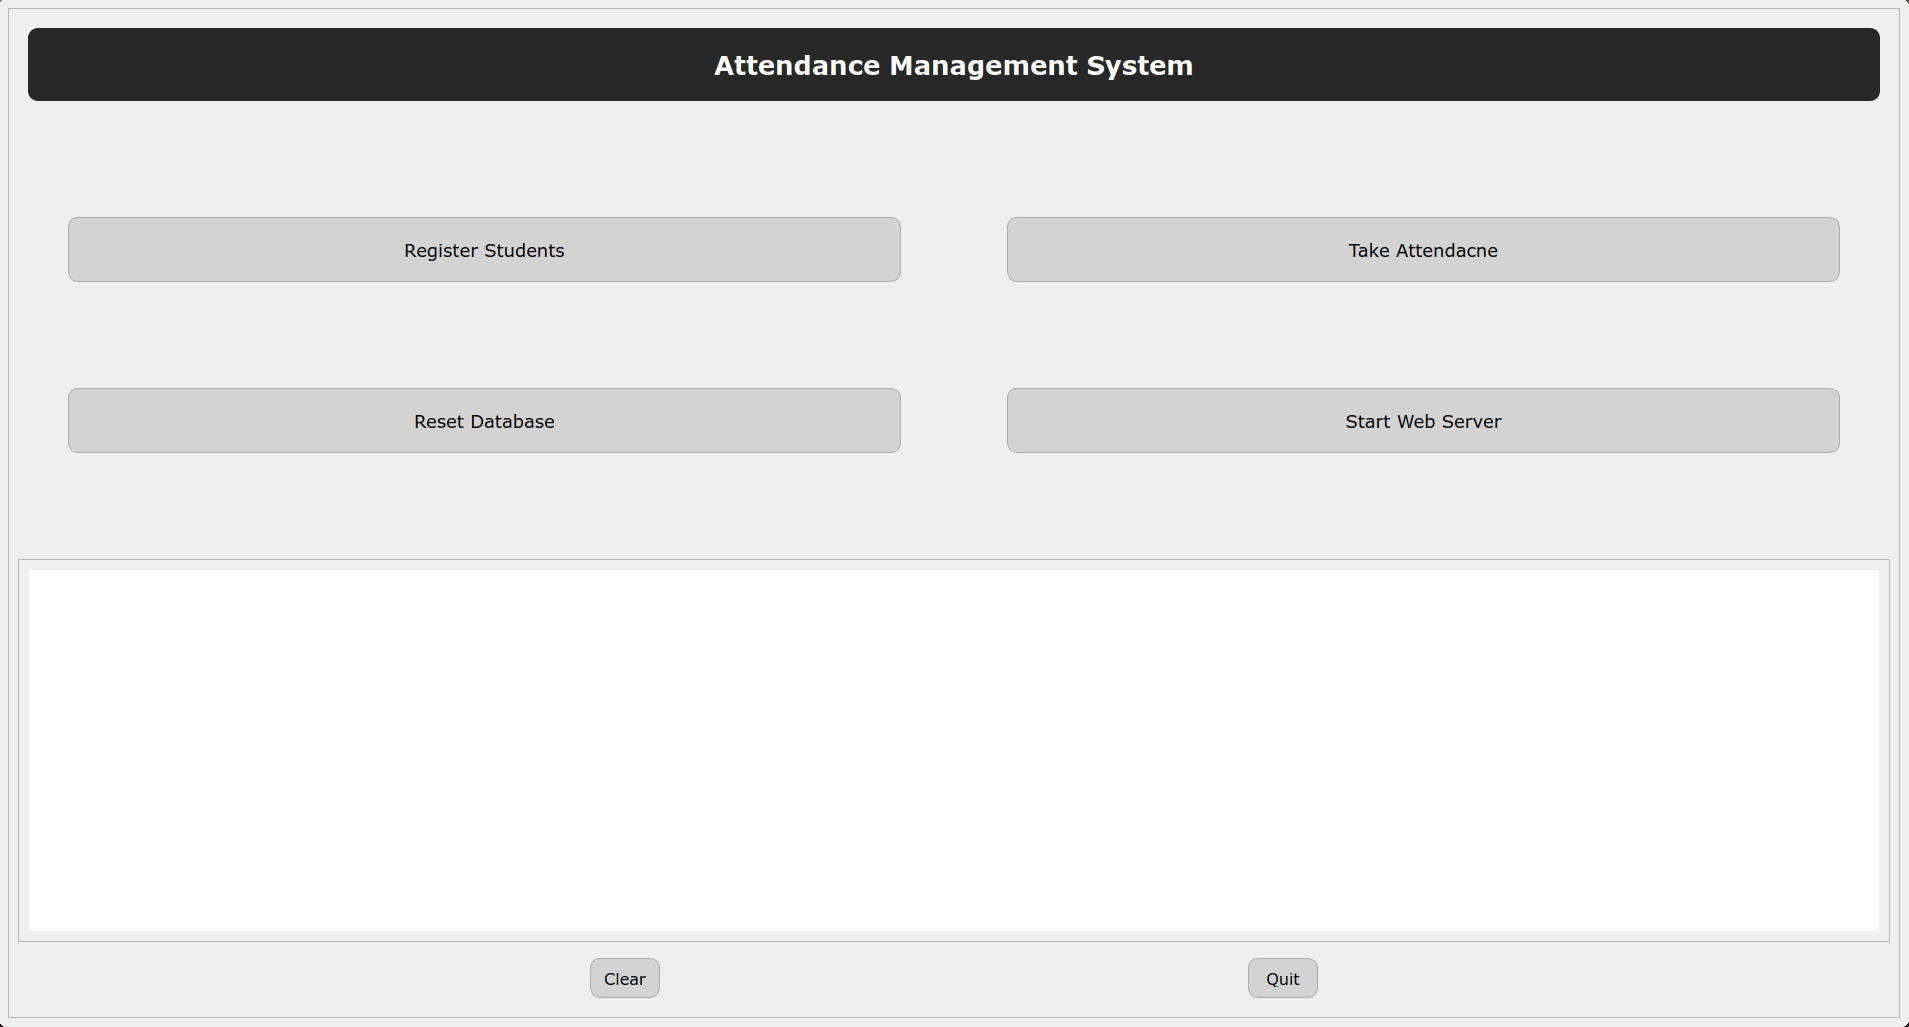
\includegraphics[scale=0.2]{images/AMSFR_Screenshot-1.png}
			\end{center}
			\caption{Graphical User Interface For Attendance Management System}
		\end{figure}

		\tikzstyle{startstop} = [rectangle, rounded corners, minimum width=3cm, minimum height=1cm,text centered, draw=black, fill=black!10]
\tikzstyle{io} = [trapezium, trapezium left angle=70, trapezium right angle=110, minimum width=3cm, minimum height=1cm, text centered, text width=3cm, draw=black, fill=black!10]
\tikzstyle{process} = [rectangle, minimum width=3cm, minimum height=1cm, text centered, text width=3cm, draw=black, fill=black!10]
\tikzstyle{decision} = [diamond, minimum width=2cm, minimum height=1cm, text centered, text width=2cm, draw=black, fill=black!10]
\tikzstyle{arrow} = [thick,->,>=stealth]

\begin{figure}[H]
	\begin{center}
		\begin{tikzpicture}[node distance=2cm]
			\node (start) [startstop] {START};
			\node (regs) [decision, below of=start, yshift=-1cm] {Registered Students};
			\node (stop) [startstop, left of=regs, xshift=-3cm] {STOP};
			\node (webs) [decision, below of=regs, yshift=-2.5cm] {Web Server};
			\node (getregs) [io, below of=webs, yshift=-1cm] {Get the name of registered students};
			\node (matchregs) [process, below of=getregs, yshift=-0.5cm] {Match the face on webcam to registered students};
			\node (ifmatch) [decision, below of=matchregs, yshift=-1cm] {If matched};
			\node (marka) [io, left of=ifmatch, xshift=-2.7cm] {Display ``Matched Name"};
			\node (markn) [io, right of=ifmatch, xshift=2.7cm] {Display ``Not Registered"};
			\node (postmatch) [process, below of=marka, yshift=-1cm] {Mark Attendence and POST the matched name to the web server};
			\node (postmatchn) [process, below of=markn, yshift=-0.5cm] {POST ``Not Registered" to the web server};
			\node (wait) [process, below of=ifmatch, yshift=-3cm] {WAIT};
			\node (stop2) [startstop, below of=wait, yshift=0.4cm] {STOP};

			\draw [arrow] (start) -- (regs);
			\draw [arrow] (regs) -- node[anchor=south] {NO} (stop);
			\draw [arrow] (regs) -- node[anchor=east] {YES} (webs);
			\draw [arrow] (webs) -| node[anchor=south west] {NO} (stop);
			\draw [arrow] (webs) -- node[anchor=east] {YES} (getregs);
			\draw [arrow] (getregs) -- (matchregs);
			\draw [arrow] (matchregs) -- (ifmatch);
			\draw [arrow] (ifmatch) -- node[anchor=south] {YES} (marka);
			\draw [arrow] (ifmatch) -- node[anchor=south] {NO} (markn);
			\draw [arrow] (marka) -- (postmatch);
			\draw [arrow] (markn) -- (postmatchn);
			\draw [arrow] (postmatch) |- (wait);
			\draw [arrow] (postmatchn) |- (wait);
			\draw [arrow] (wait) -- (stop2);
		\end{tikzpicture}
	\end{center}
	\caption{Attendance Management System Using Python}
\end{figure}


	\item LED Indicator Using Raspberry Pi Pico WH.
		\par This methodology outlines the steps to implement and deploy a MicroPython-based attendance system using a Raspberry Pi Pico WH microcontroller. The system connects to a server over WiFi, retrieves task names, queries a MongoDB database for attendance records, and provides visual and auditory feedback based on the task status.
		\begin{figure}[H]
			\begin{center}
				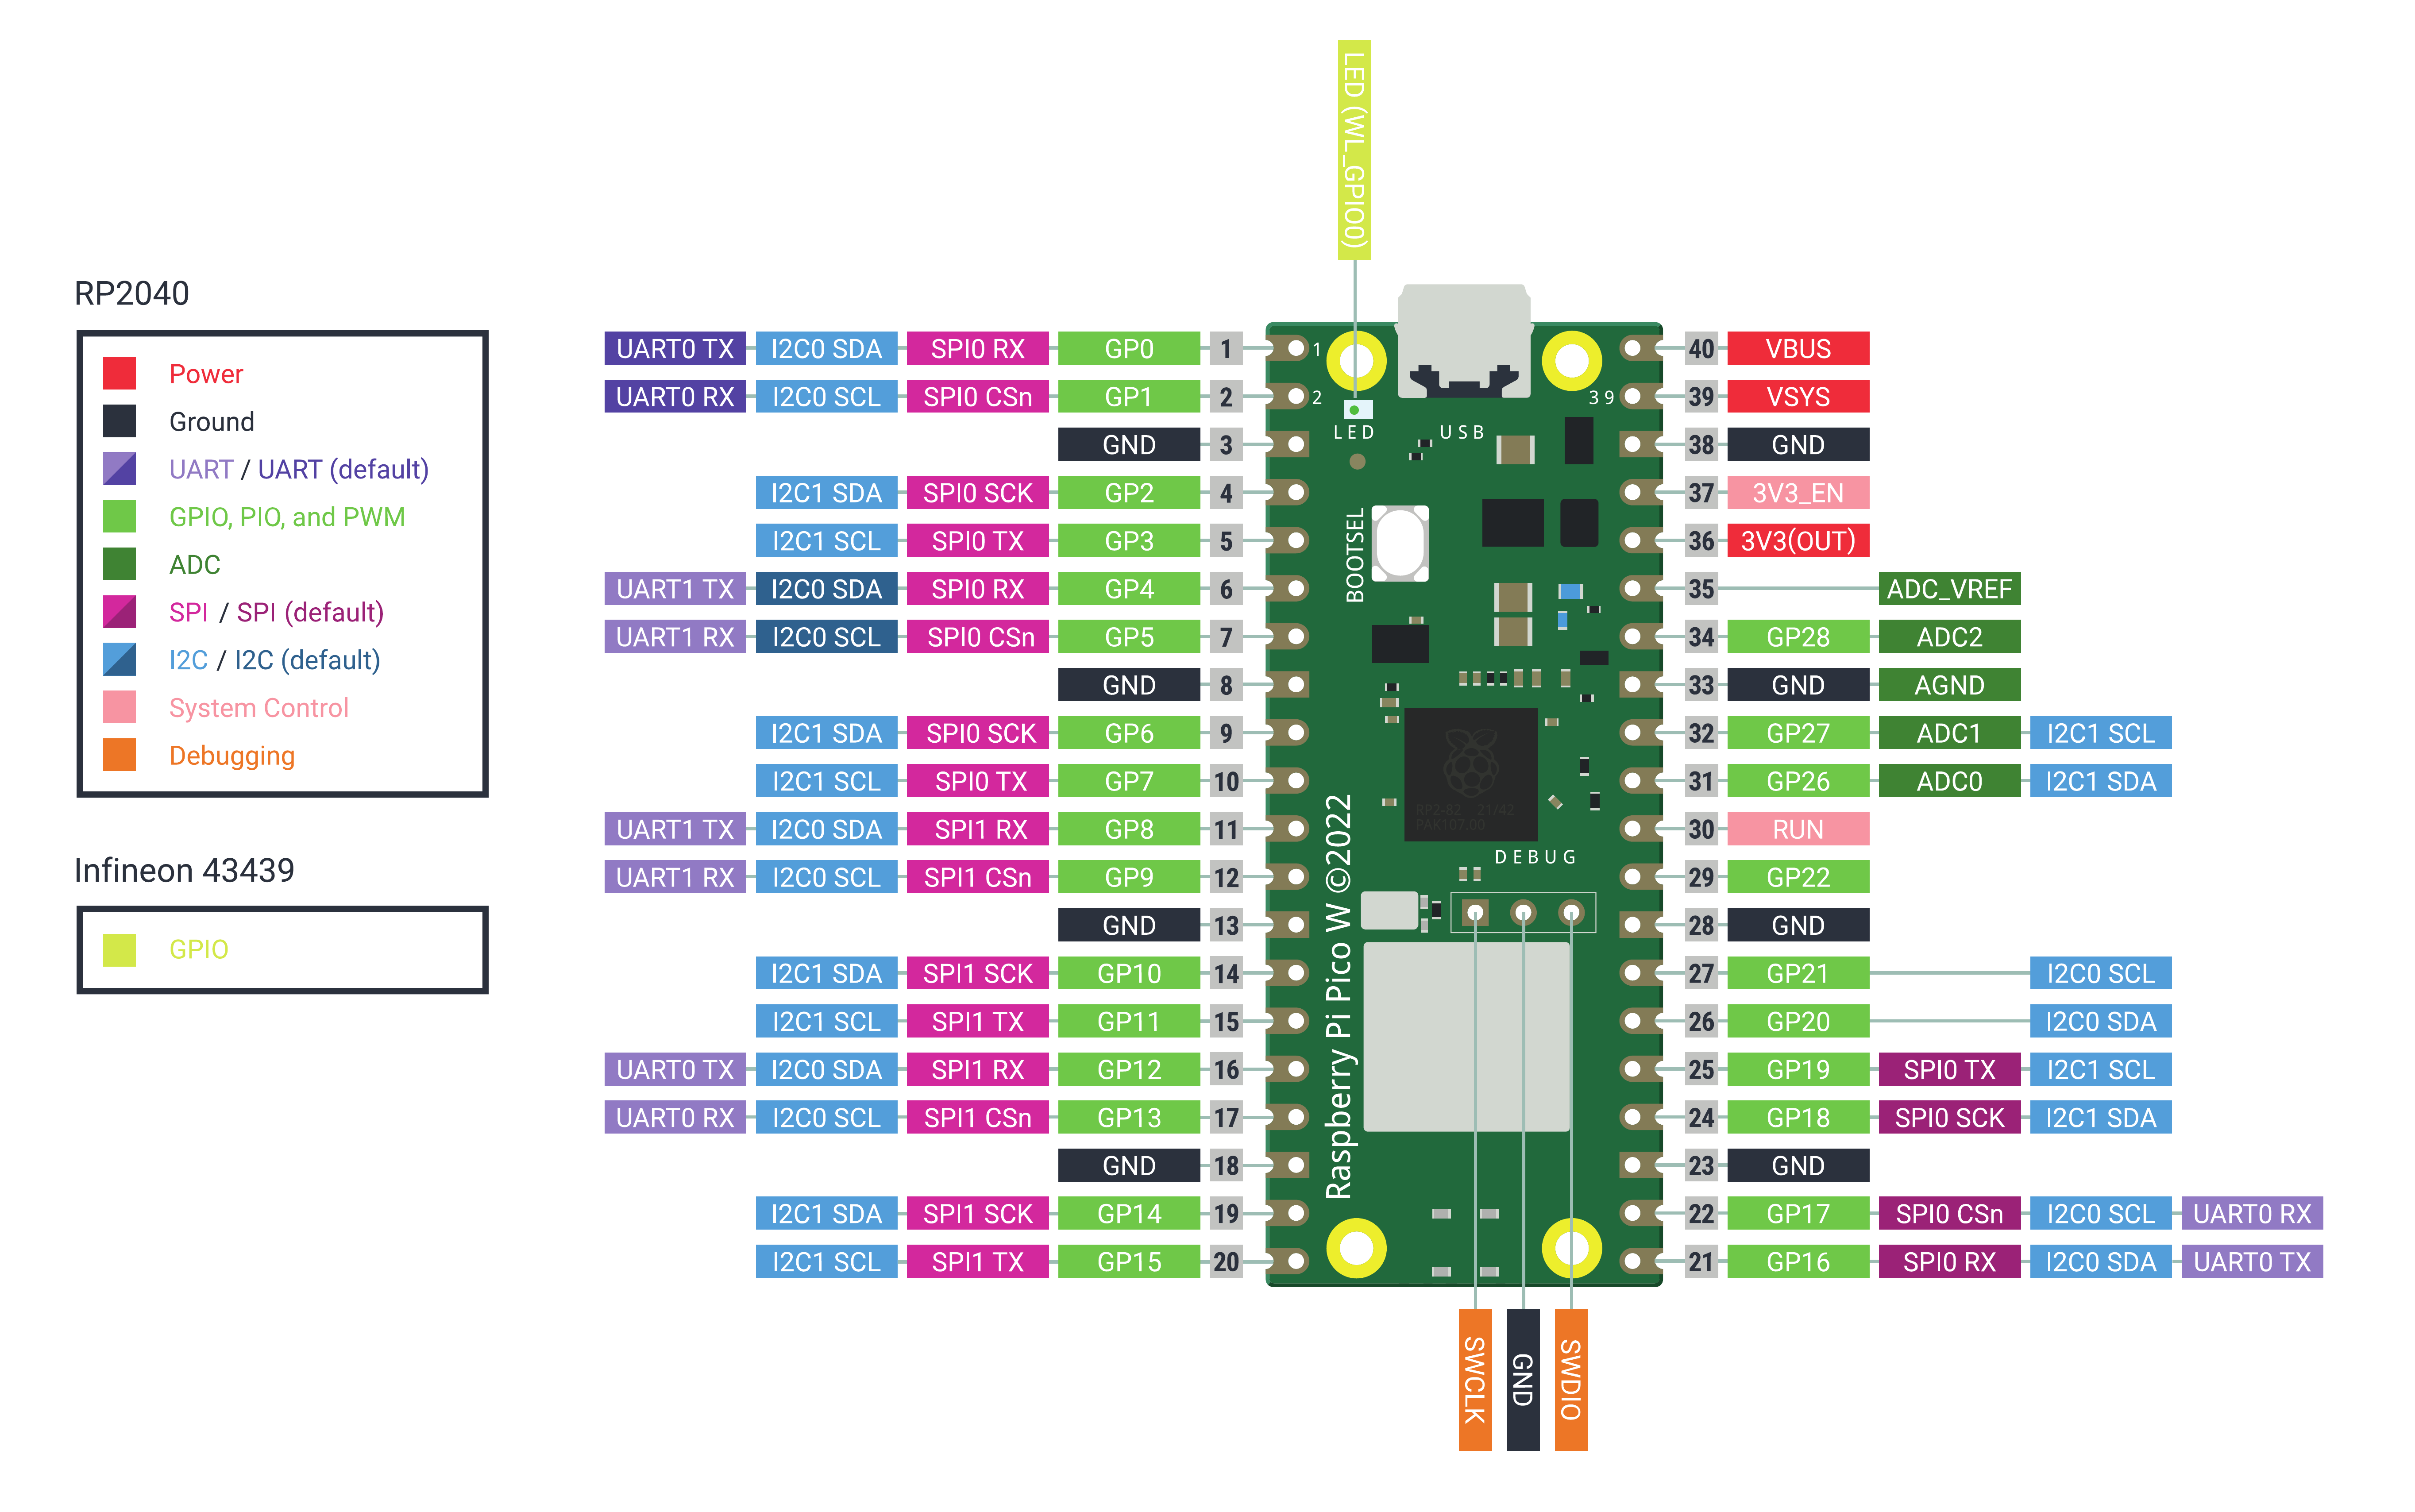
\includegraphics[scale=0.5]{images/picow-pinout.png}
			\end{center}
			\caption{Pinout Diagram of Raspberry Pi Pico WH}
		\end{figure}

		\begin{figure}[H]
			\begin{center}
				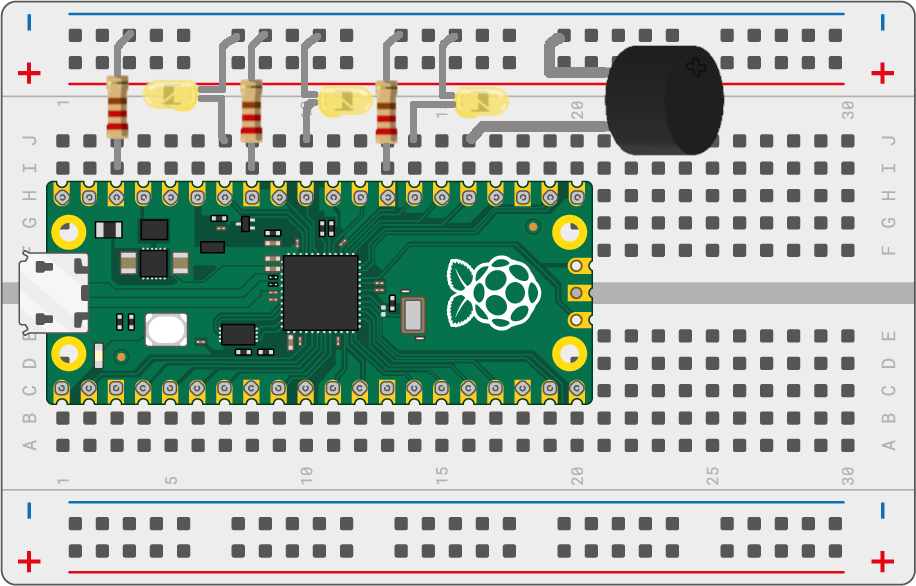
\includegraphics[scale=0.35]{images/picowh-circuit.png}
			\end{center}
			\caption{Circuit Using Raspberry Pi Pico WH}
		\end{figure}

		\newpage
		\begin{itemize}
			\item Hardware Setup.
				\begin{itemize}
					\item Microcontroller (Raspberry Pi Pico WH or ESP32)
					\item LEDs (Red, Green, Blue)
					\item Buzzer
					\item WiFi module compatible with MicroPython
					\item Breadboard, resistors, and jumper wires
				\end{itemize}
			\item Connections.
				\begin{itemize}
					\item Raspberry Pi Pico WH Pinout.
						\begin{itemize}
							\item Refer to the Raspberry Pi Pico WH pinout diagram and place the Pico WH on a breadboard.
						\end{itemize}
					\item LED Connections.
						\begin{itemize}
							\item Red LED - Anode to GP26 (Pin 31), cathode to 330-ohm resistor to ground.
							\item Blue LED - Anode to GP21 (Pin 27), cathode to 330-ohm resistor to ground.
							\item Green LED - Anode to GP28 (Pin 34), cathode to 330-ohm resistor to ground.
						\end{itemize}
					\item Buzzer Connection.
						\begin{itemize}
							\item Positive terminal to GP19 (Pin 25), negative terminal to ground.
						\end{itemize}
				\end{itemize}
			\item Software Setup.
				\begin{itemize}
					\item MicroPython Firmware - Flash MicroPython firmware onto the Raspberry Pi Pico WH.
					\item Uploading Files - Using tools like \verb|rshell|, \verb|ampy|, \verb|Thonny IDE| or any other IDE with MicroPython support to upload the necessary Python scripts (\verb|main.py|, \verb|myrequest.py|) to the microcontroller.
				\end{itemize}
			\item Implementation of the code.
				\begin{itemize}
					\item WiFi Connection - Handle connection retries and status checks.
					\item HTTP Requests - Implement a custom myrequest module to handle HTTP requests using HTTP 1.1 for MongoDB compatibility. Function to send GET and POST requests to the server.
					\item Database Interaction - Implement the find function to query the MongoDB database using the provided API key and endpoint. Define the search payload with dataSource, database, collection, filter, and projection parameters.
					\item Task Processing Logic.
						\begin{itemize}
							\item Check for new tasks from the server.
							\item Query the database for task-related information.
							\item Provide feedback based on task status using LEDs and buzzer.
						\end{itemize}
				\end{itemize}
		\end{itemize}

		\tikzstyle{startstop} = [rectangle, rounded corners, minimum width=3cm, minimum height=1cm,text centered, draw=black, fill=black!10]
\tikzstyle{io} = [trapezium, trapezium left angle=70, trapezium right angle=110, minimum width=3cm, minimum height=1cm, text centered, text width=3cm, draw=black, fill=black!10]
\tikzstyle{process} = [rectangle, minimum width=3cm, minimum height=1cm, text centered, text width=3cm, draw=black, fill=black!10]
\tikzstyle{decision} = [diamond, minimum width=2cm, minimum height=1cm, text centered, text width=2cm, draw=black, fill=black!10]
\tikzstyle{arrow} = [thick,->,>=stealth]

\begin{figure}[H]
	\begin{center}
		\begin{tikzpicture}[node distance=2cm]
			\node (start) [startstop] {START};
			\node (conwifi) [process, below of=start] {Connect to WiFi};
			\node (ifwifi) [decision, below of=conwifi, yshift=-1cm] {if true or false};
			\node (wifiy) [process, right of=ifwifi, xshift=2.5cm] {Check for POST request in Web Server};
			\node (wsy) [decision, below of=wifiy, yshift=-1.5cm] {if true or false from database};
			\node (noreg) [decision, left of=wsy, xshift=-2.5cm, yshift=-4cm] {if ``Not Registered"};
			\node (none) [decision, below of=noreg, yshift=-2cm] {if ``NONE"};
			\node (name) [decision, below of=none, yshift=-1.6cm] {if ``Match"};
			\node (redl) [io, right of=noreg, xshift=3cm] {Red LED with Buzzer};
			\node (yell) [io, right of=none, xshift=3cm] {Yellow LED with Buzzer};
			\node (greenl) [io, right of=name, xshift=3cm] {Green LED with Buzzer};

			\draw [arrow] (start) -- (conwifi);
			\draw [arrow] (conwifi) -- (ifwifi);
			\draw [arrow] (ifwifi) -- node[anchor=south] {YES} (wifiy);
			\draw [arrow] (ifwifi.west) -| ++(-0.5cm,0) -- node[anchor=south west] {NO} ++(-0.5cm, 0) |- (conwifi.west);
			\draw [arrow] (wifiy) -- (wsy);
			\draw [arrow] (wsy) -| node[anchor=north west] {YES} (noreg);
			\draw [arrow] (wsy.east) |- ++(0.5cm,0) -- node[anchor=south east] {NO} ++(0.5cm, 0) |- (wifiy.east);
			\draw [arrow] (noreg) -- (none);
			\draw [arrow] (none) -- (name);
			\draw [arrow] (name.south) |- ++(8cm, -0.5cm) |- (wsy.south);
			\draw [arrow] (noreg) -- (redl);
			\draw [arrow] (none) -- (yell);
			\draw [arrow] (name) -- (greenl);
		\end{tikzpicture}
	\end{center}
	\caption{Raspberry Pi Pico WH Running MicroPython}
\end{figure}

\end{enumerate}

\section{Tools And Technologies}
\begin{itemize}
	\item Raspberry Pi Pico WH - A microcontroller board with built-in WiFi capabilities, ideal for IoT projects. It is used to control the LEDs and buzzer based on the results of the facial recognition system.
	\item LEDs (Red, Green, Blue) - Light-emitting diodes used to provide visual feedback. The colors are used to indicate different statuses, viz.
		\begin{itemize}
			\item Red - Error or rejection.
			\item Green - Successful attendance marking.
			\item Blue - Server connection issues or other notifications.
		\end{itemize}
	\item Buzzer - An audio device that provides auditory feedback. Different tones and sequences indicate various statuses such as errors, rejections, or successful attendance marking.
	\item Resistors (330 ohms) - Used to limit the current flowing through the LEDs to prevent damage. Each LED is connected to a resistor to ensure safe operation.
	\item Breadboard and jumper wires - A breadboard is used to build the circuit without soldering, and jumper wires are used to make connections between the components and the Raspberry Pi Pico WH.
	\item WiFi module compatible with MicroPython - Enables the Raspberry Pi Pico WH to connect to a WiFi network. This is necessary for communication with the web server and the MongoDB database.
	\item Webcam for facial recognition - Captures images of faces for the facial recognition process. The images are analyzed to match against the registered faces stored in the system's database.
\end{itemize}

\section{Advantages}
\begin{itemize}
	\item Reduces the need for physical contact, which is especially beneficial for hygiene and health safety.
	\item Quickly records attendance, saving time for both administrators and users.
	\item Lessens the workload on administrative staff by automating attendance tracking and reporting.
	\item Eliminates the need for paper-based attendance records.
\end{itemize}

\section{Disadvantages}
\begin{itemize}
	\item Potential invasion of privacy due to the collection and storage of biometric data.
	\item Significant upfront investment required for hardware and software.
	\item System reliability is dependent on technology and can be affected by technical issues.
	\item Risk of inaccuracies due to bias in facial recognition algorithms.
\end{itemize}

\section{Applications}
\begin{itemize}
	\item Schools, colleges, and universities can use facial recognition to track student and staff attendance.
	\item Businesses can implement the system to monitor employee attendance and working hours.
	\item Hospitals and clinics can use facial recognition for staff attendance and patient check-ins.
	\item Government offices and public sector organizations can implement the system for employee attendance and visitor management.
	\item Large-scale events, conferences, and seminars can use facial recognition for attendee check-ins.
\end{itemize}

\chapter{Result and Discussion}
\section{Result}
\par The Attendance Monitoring System Using Facial Recognition project is designed to streamline attendance management using facial recognition technology. This system involves both a GUI application running on a standard computer and a MicroPython-based setup on a Raspberry Pi Pico WH microcontroller for physical feedback.

\begin{enumerate}
	\item \textbf{Facial Recognition Accuracy} - Facial recognition achieved an average of 80\% for facial images.
	\item \textbf{User Interaction} - User can effectively access features using graphical user interface for registration, recording attendance.
	\item \textbf{Performance} - The program runs with minimum latency in processing images and storing data.
	\item \textbf{Accessibility} - Storing data in a cloud has lead to least or less errors when compared to manual recording of attendance.
	\item \textbf{Security} - With facial recognition there is noticeably less human error and provides security and ease of recording attendance.
\end{enumerate}

\section{Discussion}
\par Implementing an attendance monitoring system using facial recognition and IoT technology presents both exciting opportunities and significant challenges. This discussion explores the implications, benefits, and potential hurdles associated with such a system.

\begin{itemize}
	\item \textbf{User Experience} - The user experience is designed to be seamless and efficient, reducing the time and effort required for attendance management.
	\item \textbf{Educational Impact} - Students gain practical experience with facial recognition technology, MicroPython programming, and hardware integration. The project helps develop skills in computer vision, database management, and IoT (Internet of Things) applications.
	\item \textbf{Future Improvements} - Developing a mobile app version for more flexible and accessible attendance management. Implementing advanced facial recognition algorithms to improve detection accuracy in diverse lighting and environmental conditions.
	\item \textbf{Technical Challenges} - Maintaining stable and reliable WiFi connections for real-time communication between the microcontroller and the server.
\end{itemize}

\newpage
\chapter{Conclusion and Future Scope}
\section{Conclusion}
\par The integration of facial recognition technology with IoT devices for attendance monitoring represents a significant advancement in how attendance is tracked and managed. This innovative approach offers numerous benefits, including enhanced accuracy, improved efficiency, and a more streamlined process compared to traditional methods. By automating attendance recording through contactless facial recognition, organizations can reduce errors, save time, and minimize administrative burdens.\\
\par Despite its advantages, the implementation of such a system comes with challenges that must be carefully managed. Privacy and data security concerns, accuracy and reliability issues, and the need for scalable infrastructure are critical factors that need to be addressed to ensure the system's success. Additionally, achieving user acceptance and navigating the legal landscape are essential for the system's effective deployment.\\
\par Looking towards the future, the potential for advancements in artificial intelligence, cloud computing, and IoT technologies promises further improvements in the functionality and efficiency of attendance monitoring systems. Integration with other biometric systems, real-time analytics, and enhanced security measures will likely drive the evolution of these systems, making them more adaptable and effective across various applications.\\
\par In summary, an attendance monitoring system utilizing facial recognition and IoT has the potential to transform how attendance is managed, offering a modern solution to longstanding challenges. With careful consideration of the associated challenges and a focus on future innovations, these systems can deliver substantial benefits, paving the way for more accurate, efficient, and secure attendance management solutions in diverse settings.\\

\newpage
\section{Future Scope}
\par The future scope of attendance monitoring systems using facial recognition and IoT is vast and promising, with several potential advancements and integrations that can further enhance their effectiveness and utility.

\begin{enumerate}
	\item \textbf{3D Facial Recognition} - Explore 3D facial recognition technology to enhance recognition accuracy by capturing facial features in three dimensions, which is less affected by changes in lighting and angles.
	\item \textbf{Distributed System} - Implement a distributed system architecture where multiple Raspberry Pi devices can work together to manage attendance in larger environments, such as multiple classrooms or an entire school.
	\item \textbf{QR Code Integration} - Integrate QR code scanning as an alternative or supplementary method for attendance marking, enabling students to quickly register their attendance using mobile devices.
	\item \textbf{Customizable Alerts} - Allow users to customize alerts and notifications for different attendance scenarios, such as absences, late arrivals, or special events.
	\item \textbf{Data Encryption} - Implement robust data encryption methods for storing and transmitting facial recognition data to ensure privacy and security.
	\item \textbf{Calendar Integration} - Sync the attendance system with calendar applications to automatically adjust for holidays, special events, and schedule changes.
	\item \textbf{Outdoor Usage} - Adapt the system for outdoor usage, ensuring reliable performance under varying weather conditions. This could involve ruggedizing the hardware components and using cameras with better dynamic range.
	\item \textbf{Night Mode} - Implement a night mode with infrared cameras to facilitate attendance tracking in low-light conditions or during evening classes.
\end{enumerate}

\par By addressing these future improvements, the Attendance Management System can become more robust, user-friendly, and versatile, better meeting the needs of educational institutions and enhancing the overall user experience.

\newpage
\nocite{*}
\printbibliography[heading=bibintoc, title={References}]

\end{document}
